
\section{Technical standards}
In this section we define explicitly the technical data exchange
formats defined in the previous subsections.

%%%%%%%%%%%%%%%%%%%%%%%%%%%%%%%%%%%%%%%%%%%%%%%%%%%%%%%%%%%%%%%%%%%%%%%%%%%%%%%
\subsection{File encoding and data storage format per type}
Below we propose a JSON format \citep{ecma2013json} for exchanging data
validation reports.  Although it is a textual format, the JSON standard does
not impose restrictions on the encoding used. It is left explicitly to
standards built upon JSON to define an encoding \citep[pp ii]{ecma2013json}. In
this standard we follow the currently most widely applied standard (see
Figure~\ref{fig:encoding}) with the following demand.

\begin{center}
\captionof{table}{File encoding used for validation reports}
\label{tab:encoding}
\begin{tabular}{|p{0.97\textwidth}|}
\hline
Validation reports  are encoded in \code{UTF-8}.\\
\hline
\end{tabular}
\end{center}

\begin{figure}[t]
\centering
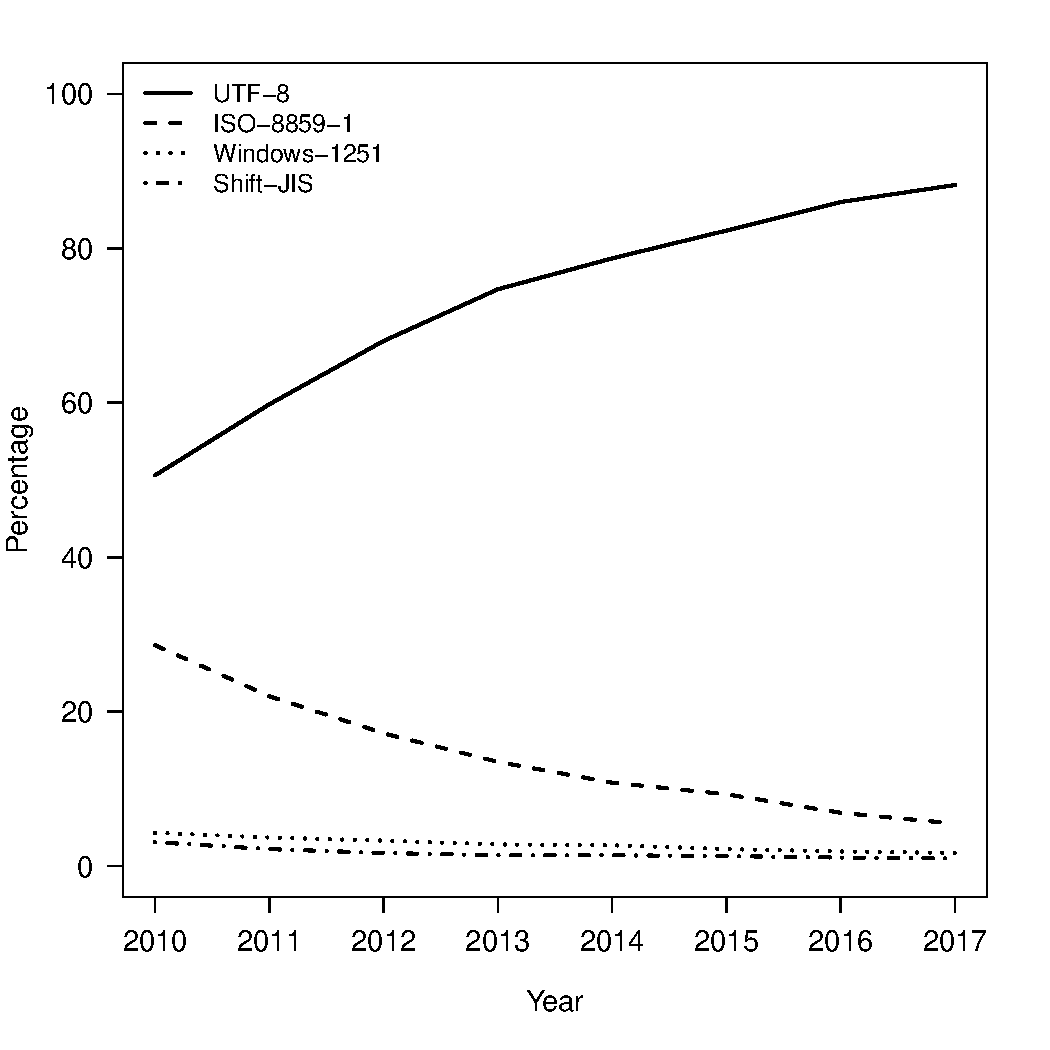
\includegraphics[width=0.7\textwidth]{fig/encoding_use.pdf}
\caption{Percentages of encoding standards used on the web \citep{w3techs2017}.}
\label{fig:encoding}
\end{figure}

The different data types within a file are to be formatted according to
commonly used standards where possible. In particular, data in validation
reports are encoded as stated in Table~\ref{tab:dataformat}.
\begin{center}
\captionof{table}{Format of data types in validation reports.}
\begin{tabular}{|lp{0.92\textwidth}|}
\hline
1&Numbers are encoded in a valid decimal ISO/IEC/IEEE 60559:2011 (IEEE 754) format
\citep{ieee:2008}. \\
2&Date-time data shall be denoted in ISO 8601 format \code{YYMMDDTHHmmss+HHMM} \citep{iso2004data}. \\
\hline
\end{tabular}
\label{tab:dataformat}
\end{center}

%%%%%%%%%%%%%%%%%%%%%%%%%%%%%%%%%%%%%%%%%%%%%%%%%%%%%%%%%%%%%%%%%%%%%%%%%%%%%%%
\clearpage{}
\subsection{JSON messages}
To implement the basic and extended validation report we devise a simple object model
allowing for reuse of some components. Recall that the basic results are
identified as a \emph{confrontation} (Definition~\ref{def:confrontation})
and aggregates are identified as a \emph{aggregation} (Definition~\ref{def:aggregation}.
We therefore define the following objects.
\begin{align}
\label{eq:confrontation}
\textsf{confrontation} &: 
  \langle\textsf{event}, \textsf{rule}, \textsf{data}, \textsf{value}\rangle\\
\textsf{aggregation}   &:
\langle\textsf{aggregator}, \textsf{nodeset},\textsf{value}\rangle
\end{align}
The mandatory and optional subcomponents of these objects have been discussed
in Sections~\ref{sect:idevent}--\ref{sect:valres} and \ref{sect:aggregators}--\ref{sect:nodesets}.

JSON schemas that define a transmission format for these objects are given in
Listings~\ref{lst:confrontation} and \ref{lst:aggregation}, on pages
\pageref{lst:confrontation} and \pageref{lst:aggregation} of the next section
respectively. Listing~\ref{lst:exampleconfrontation} shows an example
confrontation JSON message, conforming to this standard. Note that this is not
a yet a full validation report since this would allow for multiple
confrontations to be stored.  In this example, a validation event was executed
using R version 3.4.0 on 18 May 2017 at 10:50:55, in the UTC+2 timezone (this
is CEST, summertime).  The rule is stated using syntax accepted by R package
\code{validate} version 0.1.7, and the expression is \code{income >=  0}.
Failure to pass this rule indicates an error, and there is also a short
description. The data under scrutiny is coded in a length 4 arrayt using the
$U\tau uX$ model for data identification.  In this case the household income of
household number \code{"8237193679"}, as collected during the Household survey
of 2017 amongst Dutch inhabitants was checked. The result is \code{1}, meaning
that the test is passed.
%
\begin{lstlisting}[
  frame=single
  , float=h
  , caption=An example JSON confrontation message
  , label=lst:exampleconfrontation]
{
  "event": {
    "time": "20170518T105055+02",
    "actor": "R 3.4.0",
    "agent": null,
    "trigger": null
  },
  "rule": {
    "language": "R pkg validate 0.1.7",
    "expression": "income >= 0",
    "severity": "error",
    "description": "total income must be non-negative"
  },
  "data": [
    "Dutch inhabitants",
    "Household survey 2017",
    "8237193679",
    "Household Income"
  ],
  "value": "1"
}
\end{lstlisting}
\begin{lstlisting}[
  frame=single
  , linewidth=1.1\textwidth
  , float=h
  , caption=An example JSON aggregation message
  , label=lst:exampleaggregation
  ]
{
  "aggregator": {
    "language": "R 3.4.0",
    "expression": "mean(x,na.rm=TRUE)",
    "description": "Fraction of non-NA events passing."
  },
  "nodeset": {
    "keys": [
      "x0coffee",
      "x0beefed"
    ],
    "description": "All confrontations."
  },
  "value": "0.5"
}
\end{lstlisting}

An example aggregation message is shown in
Listing~\ref{lst:exampleaggregation}.  This partial message conveys an
aggregate, computed using R 3.4.0 with the expression \code{mean(x,
na.rm=TRUE)}. According to the description this results in the fraction of
passes, computed over the values that actually resulted in a value (not \na{}).
The nodes over which this fraction is computed are identified with hexadecimal
keys \code{0xcoffee} and \code{0xbeefed}, which according to the description
corresponds to all confrontations in the complete message.
%


Now that the basic information components have been defined, we can define the
basic and extended validation report. A JSON message containing a validation
report is just an array of confrontations. The JSON schema is given in
Listing~\ref{lst:basic}.

The extended validation report represents a directed acyclic graph.  Each node
in this graph is represented as a key-value pair where the payload can either
be a confrontation, corresponding to the result of a single validation event,
or an aggregate.  Symbolically (using `$|$' to indicate `or'):
\begin{align}
\label{eq:node}
\textsf{node} &: \langle \textsf{key},\textsf{value}\rangle\textrm{, where }
\textsf{value} : \langle \textsf{confrontation} | \textsf{aggregation}\rangle.
\end{align}


\clearpage{}
%%%%%%%%%%%%%%%%%%%%%%%%%%%%%%%%%%%%%%%%%%%%%%%%%%%%%%%%%%%%%%%%%%%%%%%%%%%%%%%
\subsection{JSON Schemas}
In this subsection the JSON schemas defining the basic and extended
validation reports and their components are listed as a reference.

The full code can also be found at github:
\begin{center}
\href{https://github.com/data-cleaning/ValidatReport}{https://github.com/data-cleaning/ValidatReport}
\end{center}
%
\lstinputlisting[frame=single
  , float=h,caption=JSON schema for a confrontation object.
  , label=lst:confrontation]{../json/confrontation.json}
%
%
\lstinputlisting[frame=single
  , float=h
  , linewidth=1.1\textwidth
  , caption=JSON schema for an aggregation object..
  , label=lst:aggregation]{../json/aggregation.json}
%

%
\lstinputlisting[frame=single
  , float=h
  , caption=JSON schema for basic validation report.
  , label=lst:basic]{../json/basic_validation_report.json}
%




%
\lstinputlisting[frame=single
  , float=h
  , caption=JSON schema for extended validation report.
  , label=lst:extended]{../json/extended_validation_report.json}
%





